% !TEX TS-program = xelatex
% !TEX encoding = UTF-8 Unicode

\documentclass[a4paper,10pt,hidelinks]{article}
\usepackage{latexsym}
\usepackage{bookmark}
\usepackage[empty]{fullpage}
\usepackage{titlesec}
\usepackage{marvosym}
\usepackage[T1]{fontenc}
\usepackage{fontspec}
\usepackage{tikz}
\usetikzlibrary{shapes,calc}
\usepackage{xcolor}
\usepackage{lipsum}
\usepackage{ragged2e}
\usepackage{etoolbox}
\usepackage{ifmtarg}
\usepackage{ifthen}
\usepackage{pgffor}
\usepackage{marvosym}
\usepackage{parskip}
\usepackage[absolute,overlay]{textpos}
\usepackage[left=7.6cm,top=1cm,right=1cm,bottom=0.8cm,nohead,nofoot]{geometry}
\usepackage{fontawesome5}
\usepackage{setspace}
\usepackage{ifthen}
\usepackage{datetime}
\usepackage{enumitem}
\usepackage{graphics}
\usepackage{pdfpages}
\hypersetup{
	pdftitle={Morteza Karimi CV},
	pdfauthor={Morteza Karimi},
	pdfsubject={Morteza Karimi Web Develpoer CV},
	pdfkeywords={CV,Resume,Morteza Karimi,Web Developer,Back-end Developer,Front-end Developer},
	colorlinks=false,
	allbordercolors=white
}
\graphicspath{{images/}}
%\import{./logo2.eps_tex}{logo2.eps_tex}
%%%%%%%%%%%%%%%%%%%%%%%%%% definitions %%%%%%%%%%%%%%%%%%%%%%%%%%%%%%%%%%%%%%5
\definecolor{defaultfontcolor}{HTML}{212121}
\definecolor{white}{RGB}{224,224,224}
\definecolor{gray}{HTML}{4D4D4D}
\definecolor{bootstrapSecondary}{HTML}{6c757d}
\definecolor{sidecolor}{HTML}{212121}
\definecolor{sidetextcolor}{RGB}{224,224,224}
\definecolor{mainblue}{HTML}{5AB9EA}
\definecolor{maingreen}{HTML}{52D3AA}
\definecolor{maingray}{HTML}{B9B9B9}
\setmainfont{GT Walsheim Pro}
\newdateformat{usvardate}{%
	\monthname[\THEMONTH] \ordinal{DAY}, \THEYEAR}

\pagestyle{empty} % Disable headers and footers

\newfontfamily\janeroe{Jane Roe}

%%%%%%%%%%%%%%%%%%%%%%%%%% Margin %%%%%%%%%%%%%%%%%%%%%%%%%%%%%%%%
\setlength{\parindent}{5pt} % Disable paragraph indentation
\renewcommand{\baselinestretch}{1.3} 
\setlength{\TPHorizModule}{1cm} % Left margin
\setlength{\TPVertModule}{2cm} % Top margin

%%%%%%%%%%%%%%%%%%%%%% Profile Picture %%%%%%%%%%%%%%%%%%%%%%%%%%%%%%
\newlength\imagewidth
\newlength\imagescale
\pgfmathsetlength{\imagewidth}{3cm}
\pgfmathsetlength{\imagescale}{\imagewidth/600}
\newcommand{\profilepic}[1]{\renewcommand{\profilepic}{#1}}

%%%%%%%%%%%%%%%%%%%%%%% birthday %%%%%%%%%%%%%%%%%%%%%%%%
\newdate{birthday}{17}{06}{1994}
\newcommand{\birthdate}{\usvardate\displaydate{birthday}}

\makeatletter
%%%%%%%%%%%%%%%%%%% change default color %%%%%%%%%%%%%%%%%%%%
\newcommand{\globalcolor}[1]{%
	\color{#1}\global\let\default@color\current@color
}

%%%%%%%%%%%%%%%%%%%%%%%%%% New Commands %%%%%%%%%%%%%%%%%%%%%%%%%%
\newcommand{\resumeItem}[6][]{
	\ifthenelse{\equal{#1}{}}{\subsection*{#2}}{\subsection*{\href{#1}{#2}}}
	{\normalsize #3}\\
	\textcolor{bootstrapSecondary}{
				% \ifthenelse{\equal{#4}{}}{}{\small{#4}{ / }}
		{\small#5}\\
	}
	{#6}
}

\newcommand{\resumeSubheading}[3]{\textbf{#1} & \small\textcolor{bootstrapSecondary}{#2} \\
	{\small#3}\\
			% \ifthenelse{\equal{#1}{}}{}{\tiny{\textbf{Thesis Title:} #1 }&\\}
}
\newcommand{\resumeSubHeadingListStart}{\begin{tabular*}{\textwidth}{@{}l@{\extracolsep{\fill}}l}}
	\newcommand{\resumeSubHeadingListEnd}{\end{tabular*}}%\vspace{-5pt}}
\renewcommand{\labelitemi}{$\bullet$}
\renewcommand{\labelitemii}{$\circ$}
%%%%%%%%%%%%%%%%%%%% Side Section Rule %%%%%%%%%%%%%%%%%%%%%%%%%%%%%%%%%%55
\newcommand{\siderule}{
	\vspace*{0.5\baselineskip}
	\hrule\@height 1pt
	\vspace*{0.5\baselineskip}
}
%%%%%%%%%%%%%%%%%%%%%%%%%%% Content Item %%%%%%%%%%%%%%%%%%%%%%%%%%%%%%%%%%%%%%
\newcommand{\contactItem}[3][]{%
	\textcolor{maingreen}{\Large{#2}} &
	{
		\ifthenelse{\equal{#1}{}}
		{
			#3
		}{
			\href{#1}{#3}
		}
	}\\
}

%%%%%%%%%%%%%%%%%%%%%%%%%%%%%% Skills Item %%%%%%%%%%%%%%%%%%%%%%%%%%%%%%%%
\newcounter{circle}
\newcommand{\skillItem}[2]{%
	\textbf{#1}\hfill
	\textcolor{maingreen}{
		\setcounter{circle}{0}
		\whiledo {\value{circle} < #2}%
		{%
			\small\faCircle\,
			\stepcounter {circle}%
		}
		\whiledo {\value{circle} < 5}%
		{%
			\small\faCircle[regular]\,
			\stepcounter {circle}%
		}
	}\\
}
%%%%%%%%%%%%%%%% Profile Section in side panel %%%%%%%%%%%%%%%%%%%%%%%%%%%%%%%%%%%%%%%%
\newcommand{\makeprofile}{
	%%%%%%%%%%%%% side background %%%%%%%%%%%%%%%%%%%%%
	\begin{tikzpicture}[remember picture,overlay]
	\node [rectangle, fill=sidecolor, anchor=north, minimum width=9cm, minimum height=\paperheight + 1cm] (box) at (-6cm,2cm){};
	\end{tikzpicture}
	%%%%%%%%%%%%%%% text block %%%%%%%%%%%%%%%%%%%%%
	\begin{textblock}{5}(0.5, 0.2)
		\textcolor{sidetextcolor}{
			%%%%%%%%%%%%%%%%%%%% profile pic %%%%%%%%%%%%%%%%%%%%%%%%%%
			\ifthenelse{\equal{\profilepic}{}}{}{
				\begin{center}
					\begin{tikzpicture}[x=\imagescale,y=-\imagescale]
					\clip (600/2, 600/2) circle (600/2);
					\node[anchor=north west, inner sep=0pt, outer sep=0pt] at (1,0) {\includegraphics[width=\imagewidth]{\profilepic}};
					\end{tikzpicture}
				\end{center}
			}
			%%%%%%%%%%%%%%%%%%%% Contact Section %%%%%%%%%%%%%%%
			\section*{Contact}\siderule
			\begin{spacing}{1.5}
				\begin{tabular}{c l}
					% \contactItem{\faBirthdayCake}{\birthdate}
					% \contactItem{\faRing}{Married}
					\contactItem[tel:+989216351266 ]{\faMobile*}{+98 921 635 1266}
					\contactItem[https://goo.gl/maps/jYxSpCQwgsqPfagbA?coh=178571\&entry=tt]{\faMapMarker*}{Tehran, Iran}
					\contactItem[https://morteza-karimi.ir]{\faGlobe}{morteza-karimi.ir}
					\contactItem[mailto:me@morteza-karimi.ir]{\faEnvelope}{me@morteza-karimi.ir}
					\contactItem[https://www.linkedin.com/in/MortezaKarimi]{\faLinkedin}{MortezaKarimi}
					\contactItem[https://github.com/MortezaKarimi]{\faGithub}{MortezaKarimi}
					\contactItem[https://stackoverflow.com/users/3307768/mortie]{\faStackOverflow}{MortezaKarimi}
				\end{tabular}
			\end{spacing}
			\vspace*{-0.4\baselineskip}
			%%%%%%%%%%%%%%%%%%%% Hard Skills Section %%%%%%%%%%%%%%%
			\section*{Hard Skills}\siderule
			\vspace*{-0.4\baselineskip}
			\begin{spacing}{1.5}
				\skillItem{PHP}{4}
				\skillItem{Symfony}{4}
				\skillItem{Ansible}{4}
				\skillItem{Angular}{4}
				\skillItem{Docker}{3}
				\skillItem{JavaScript}{3}
				\skillItem{Yii2}{4}
				\skillItem{Gitlab CI/CD}{2}			
				\skillItem{Laravel}{2}
				\skillItem{Python}{2}
				\skillItem{Node.JS}{2}
				\skillItem{Tensorflow}{2}
				\skillItem{OpenCV}{2}
			\end{spacing}
			\vspace*{-2\baselineskip}
			%%%%%%%%%%%%%%%%%%% Languages Section %%%%%%%%%%%%%%%
			\section*{Soft Skills}\siderule
			\vspace*{-.4\baselineskip}
			\begin{spacing}{1}
				\begin{itemize}[leftmargin=*]
					\setlength\itemsep{-.4em}
					\item{Team Work}
					\item{Decision-making}
					\item{Problem-solving}
					\item{Time management}
					\item{Adaptability}
					\item{Critical thinking}
				\end{itemize}
			\end{spacing}
			\vspace*{-\baselineskip}
			\section*{Interests}\siderule
			\vspace*{-0.4\baselineskip}
			\begin{spacing}{1.5}
				\resizebox{\linewidth}{!}{%
					\begin{tabular}{cccc}
						\huge\faLaptopCode&
						\huge\faRunning&
						\huge\faSuitcaseRolling&
						\huge\faMugHot\\
					\end{tabular}
				}
			\end{spacing}
}
\end{textblock}
\hspace*{-1.2em}
}

\makeatother

\profilepic{morteza.jpg}
\author{Morteza Karimi}
\title{Full-Stack Developer | DevOps Engineer}

\makeatletter
%%%%% Set default color %%%%%
\AtBeginDocument{\globalcolor{defaultfontcolor}}
\begin{document}
	% 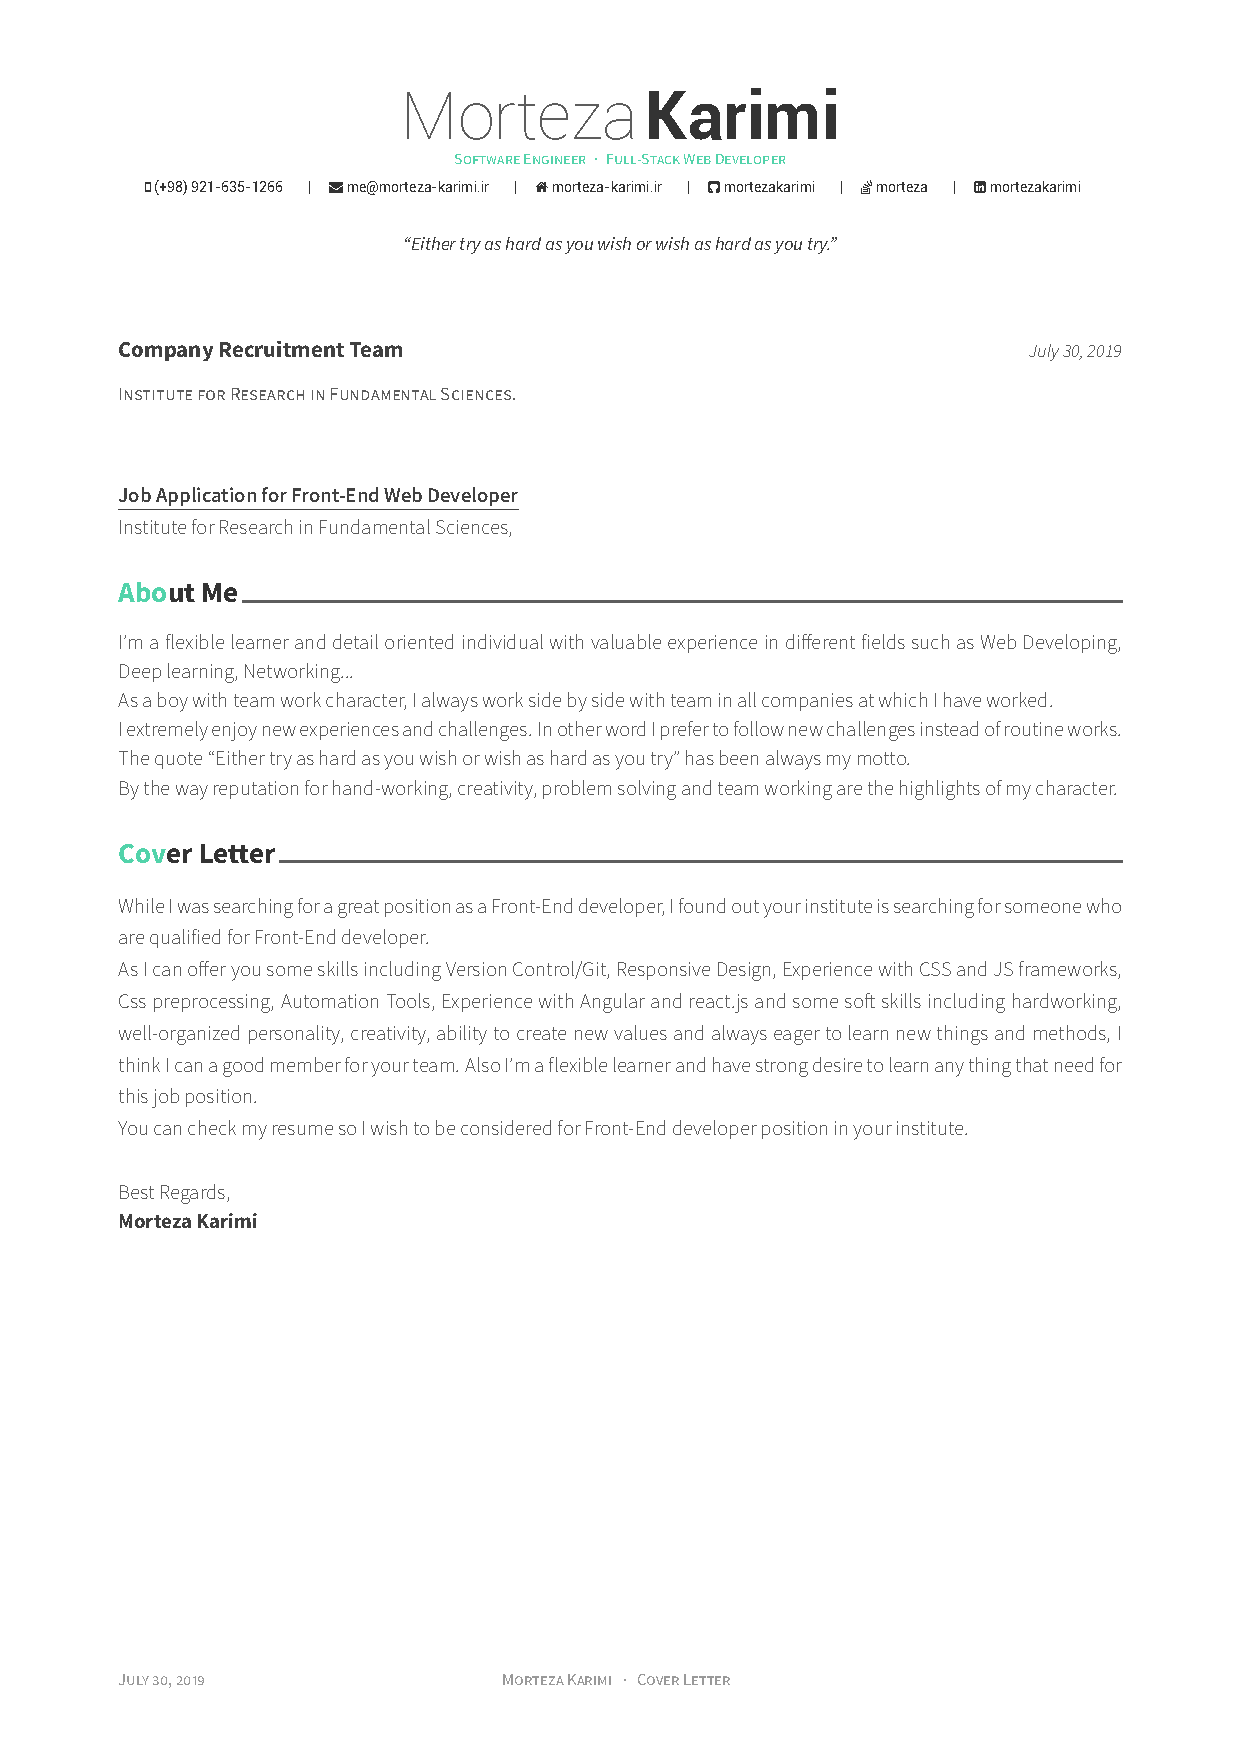
\includepdf{./CoverLetter/morteza-karimi-coverletter.pdf}
	\newpage
	\makeprofile
	{\Huge\janeroe \textbf{\@author}}\\[0.2\baselineskip]
	{\large\janeroe\@title}
	\section*{About Me}\hrule
	I am a \textbf{detail-oriented} and \textbf{flexible learner} with extensive experience in various fields such as \textbf{Web Development}, Deep Learning, Networking, \textbf{Linux}, \textbf{Windows}, and more. As a \textbf{team player}, I enjoy working alongside others to achieve common goals. I am always seeking new experiences and challenges, preferring to take on new and exciting projects rather than routine work. My reputation for \textbf{creativity}, \textbf{problem-solving}, \textbf{hard work}, and teamwork is a testament to my character. I have mastered \textbf{Symfony framework} and \textbf{Node.js}, which has given me the ability to develop and improve complex projects. For instance, in my previous job, I worked on \textbf{Microservice architecture} and introduced modern and automated solutions using \textbf{Docker}, \textbf{Ansible}, and \textbf{Gitlab CI/CD} to increase productivity and efficiency. My passion for learning led me to expand my skill set by mastering \textbf{Angular}, which elevated my position in Bugloss Company from a backend developer to a full-stack developer. During my time at Heyzha Company, I designed and developed complicated portals using \textbf{Laravel} and \textbf{Yii2} frameworks.
	
	\vspace*{-1\baselineskip}
	\section*{Experience}\hrule
	\resumeItem[https://bugloos.com/]{Bugloos}{Junior DevOps Engineer}{Iran, Tehran}{2021 - Present}{
		As a Fullstack Developer, I felt the need to research and work in the DevOps field. So, after some time, I started working as a Junior DevOps Engineer with the Bugloos company. I supervised the development and operation of the projects and tried to make some automatic solutions in the project architecture. To reduce the volume of repetitive daily tasks, I used Gitlab CI/CD, which helped the company and project to develop and improve.
	}
	\resumeItem[https://bugloos.com/]{Bugloos}{Full-Stack Web developer}{Iran, Tehran}{2020 - Present}{
		After working as a Backend Developer for 6 months, I felt the need to learn Angular to develop the company's project faster and better. I started to learn Angular and worked on different case studies until I had mastered it. This effort helped me to improve my job position in Bugloos from a Backend Developer to a Fullstack Developer. I shared my knowledge with my teammates and tried to make a better structure for developing the company's project, which resulted in a good impact on the quality of work in each release.
	}
	
	\newpage
	\makeprofile
	\resumeItem[https://bugloos.com/]{Bugloos}{Back-End Web developer}{Iran, Tehran}{2019 - 2020}{
		I started my work at Bugloos as a Backend Developer, where I worked on various projects with different domains, such as e-commerce and portals. My responsibilities included improving project calculation algorithms, enhancing query response time, and also updating deprecated bundles and extensions. Additionally, I worked on improving the workflow for the projects, which resulted in more efficient releases.
	}
	\resumeItem[http://heyzha.ir/]{Heyzha Programming Co}{Web Application Developer}{Iran, Sabzevar}{2017 - 2019}{
		I had the opportunity to work on numerous projects, which proved to be a turning point in my career. My work initially involved resolving issues on a website using Laravel framework. I also developed other websites utilizing Yii2 framework, resulting in a significant 33\% improvement across all Heyzha company projects. This led to a considerable increase in the company's income, and its business continued to experience an upward trend. The experience allowed me to tackle complex challenges in designing intricate portals, which further developed my skill set as a Web Developer. Overall, my time at Heyzha was an invaluable experience that sharpened my expertise in web development and enhanced my problem-solving abilities.
	}
	
	\resumeItem[http://khayyam.ac.ir/]{Khayyam University of Mashhad}{Back-End Web developer}{Iran, Mashhad}{2014 - 2016}{
		As a Back-End Web Developer at Khayyam University of Mashhad, I developed a game project called "tik-tak-toe" using node.js platform and socket.io library for IOS app. Additionally, I led a team in developing the university culture center website, leveraging my previous experience in using node.js and PHP together in my bachelor's final project.
	}
	\resumeItem{Freelance Experience}{Full-Stack Web developer}{Iran, Mashhad}{2012 - Present}{
		\begin{itemize}[leftmargin=*]
			\item Promac Co.\\
			For the first time I used my admin panel in developing this website, so it followed a great impact and it was the satisfaction of employer.
			\item Rastegary charity website\\
			It's one of my freelance works in the early years of my work field of web developing.\\ I tried to use PHP MVC framework Yii And UI framework Bootstrap in this web project.\\
			\newpage
			\makeprofile
			\hspace*{.4em}
			The first ideas of building my custom admin module for the next projects was occurred during developing this project that was very useful for my future projects.
			\item Variable project\\
			I've done different kind of student projects that included website design and android application.\\
			I worked with electron framework, Qt C++ framework, python language and many other techniques in these projects.
		\end{itemize}
	}
	\section*{Volunteer Experience}\hrule
	\resumeItem{Artificial Intelligence projects}{Programmer}{}{2017 - Present}{
		Because of my intrest in Image Processing field, voluntary I worked on image processing projects.\\Also based on my information about deep learning I started working on a project, that is about forecasting financial markets which is currently underway.}
	\resumeItem[https://morteza-karimi.ir/gentelella-rtl/public/]{Create RTL template based on Gentelella theme}{Front-End \& Translate}{}{2014 - Present}{
		Sharing my abilities and information in translating and RTL on open source template was one of my great work experience.\\By searching in google I found out a useful template so I worked on it because having good and free template could be useful for web developers.\\ I got familiar with different tools in this project and got many feedback from many people all around the world that helped me in developing this project.  
	}
	
	\resumeItem[https://valencia.ir/]{Valencia fan club website in Iran}{Full-Stack Web developer}{}{2014}{
		I started my first work experience in field of ``web developing" with designing 0 to 100 Valencia fan club website. I had a serious plan for developing this website that led to my employer satisfaction. I used Yii framework for this website to create complicated system such as like, comment and ... efficiently.
	}
	\resumeItem{Web Development Teacher}{Teacher}{}{2014 - 2019}{I always like to share my information with others so I like to have some experiences in designing open source projects or teaching my information to others. So I decided to  schedule and plan some courses to teach web development lessons to my students.}

	\newpage
	\makeprofile

	\section*{Education}\hrule
	\resumeSubHeadingListStart
	\resumeSubheading{Shahrood University of Technology}{2017 - 2019}{Master of Science in Artificial Intelligence; GPA: 3.77 (16.46/20)}
	\small\textcolor{bootstrapSecondary}{Was unable to complete my thesis due to mandatory military service obligations.}
	\\
	\resumeSubheading{Khayyam University of Mashhad}{2012 - 2017}{Bachelor of Engineering in Software Engineering; GPA: 3.17 (15.47/20)}
	\resumeSubHeadingListEnd
\end{document}